\chapter{Indledning}
\label{ch:indledning}
\mnote{Christian Klim Hansen}

% Note om hvad der skal stå i dette afsnit her.

Følgende rapport er skrevet i forbindelse med vores afsluttende
projekt i faget El-teknik.  Vi har fået udleveret tre mulige temaer,
hvor vi har valgt at arbejde med temaet Robotteknologi, som omfatter
følgende:

\begin{itemize}
\item \texttt{Udvikling af udstyr med funktioner af robotagtig karakter}
\item \texttt{Dette udstyr skal virke uden menneskelig indgriben}
\end{itemize}

Vi ønsker, at opfylde disse krav ved at lave en plotter, som aflæser
data fra et SD-kort. Plotteren har til formål at tegne en figur på et
stykke A4-papir (se afsnit \vref{sc:specificering af krav}.
\fixme{Kjærgaard:referer til kravspecifikation}. Vi
har haft i alt 100 timer pr. person fordelt ud over 10 uger. Vi har
fået stillet 300 kr. pr. person til rådighed i dette projekt til fri
benyttelse, så længde at det har en tydelig relevans for vores
projekt. Samtlige indkøb skal godkendes af læreren.


\section{Overordnede produktkrav}

Vores produkt skal indeholde følgende elementer for at overholde
produktkravene:

\begin{itemize}
\item Der skal indgå mindst et elektrisk kredsløb med passive og
  aktive komponenter udover MCU'en
\item Der skal designes printlayout vha. CAD
\item Der skal anvendes mindst én MCU
\item Der skal benyttes avancerede funktioner i MCU'en, som f.eks.:
  \begin{itemize}
  \item Interrupt
  \item Timer
  \item Tæller
  \item U(S)ART eller ADC
  \end{itemize}
\end{itemize}


\section{Specificering af Krav}
\label{sc:specificering af krav}
\fixme{Andet navn?}
\mnote{Fælles}

Vi vil lave en plotter, som opfylder følgende specifikationer:

\begin{itemize}
\item Plotteren skal tegne en figur, som vi har tegnet på computer
  \begin{itemize}
  \item Skal tegne på et stykke A4-papir
  \item Fungere uden at en computer er tilsluttet
  \item Læse data fra SD-kort
  \end{itemize}
\item Kunne forstå følgende elementer af HPGL:
  \begin{itemize}
  \item Rette linier
  \item Cirkler
  \end{itemize}
\item Anvende en AVR-processor
\item Bruge en pen til at tegne
  % \begin{itemize}
  % \item Bemærk at der ikke skal benyttes blyant eller kuglepen
  % \end{itemize}
\item Styre hastigheden af pennen meget præcist
  \begin{itemize}
  \item Med software skal vi gøre optimalt nytte af stepmotorenes præcision
  \end{itemize}
\item Kunne lave nødstop og restart med knapper
  % \item Vise status af tegneforløb på LCD-display eller med lysdioder
\item Kunne gå i nulstillingsposition (et sted hvor maskinen ved den
  så er) ved tryk på en trykknap
\item Den mekaniske konstruktion skal ligne figur\vref{fig:plotterskitse}
  \mnote{
    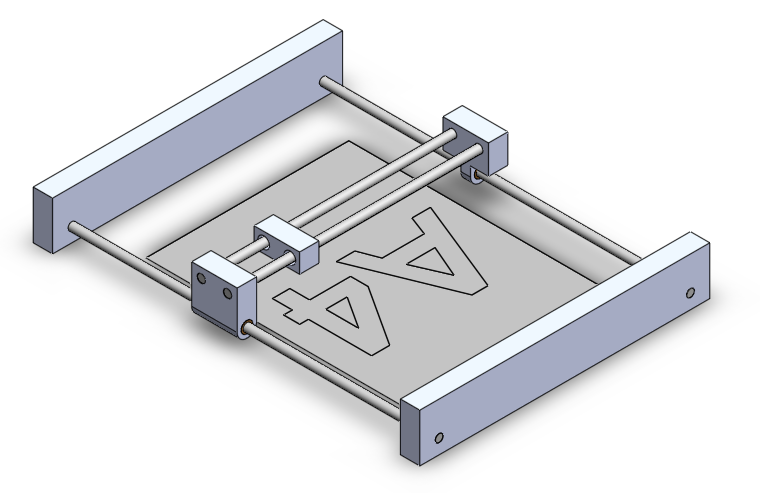
\includegraphics[width=\marginparwidth]{img/plotterskitse}
    \captionof{figure}{Skitse af konstruktion}
    \label{fig:plotterskitse}
  }
\item Bruge tandrem til at trække x- og y-akserne
  \begin{itemize}
  \item Tandremmene skal være forbundet med et par stepmotorer
  \end{itemize}
\item Pennen kan løftes og sænkes
\end{itemize}

%%% Local Variables: 
%%% mode: latex
%%% TeX-master: "../master"
%%% End: 